\documentclass[12pt]{article}

\usepackage{sbc-template}

\usepackage{graphicx,url}
\usepackage{float}
\usepackage[brazil]{babel}   
%\usepackage[latin1]{inputenc}  
\usepackage[utf8]{inputenc}  
% UTF-8 encoding is recommended by ShareLaTex
\usepackage{xcolor}
% Definindo novas cores
\definecolor{verde}{rgb}{0.25,0.5,0.35}
\definecolor{jpurple}{rgb}{0.5,0,0.35}
% Configurando layout para mostrar codigos Java
\usepackage{listings}


\bibliographystyle{ieeetr}


\lstset{
	language=Java,
	basicstyle=\ttfamily\small, 
	keywordstyle=\color{jpurple}\bfseries,
	stringstyle=\color{red},
	commentstyle=\color{verde},
	morecomment=[s][\color{blue}]{/**}{*/},
	extendedchars=true, 
	showspaces=false, 
	showstringspaces=false, 
	numbers=left,
	numberstyle=\tiny,
	breaklines=true, 
	backgroundcolor=\color{cyan!10}, 
	breakautoindent=true, 
	captionpos=b,
	xleftmargin=0pt,
	tabsize=4
}
\pagestyle{empty}
     
\sloppy
	\title{Sistema Cliente Para Conexão FTP  \\ Exercício Computacional I - Redes de Computadores}

\author{Rafael Gonçalves de Oliveria Viana\inst{1} }


\address{Sistemas de Informação -- Universidade Federal do Mato Grosso do Sul
	(UFMS)\\
  	Caixa Postal 79400-000 -- Coxim -- MS -- Brazil
  \email{rafael.viana@aluno.ufms.br}
}

\begin{document} 

\maketitle

     
\begin{resumo} 	
  Este relatório descreve como foi implementado um sistema cliente com interface gráfica para conexão FTP, utilizando JavaFX em conjunto do Apache Commons Net 3.6, uma biblioteca de conexão FTP.
\end{resumo}


\section{JavaFX}

Foi escolhido o JavaFX para criar uma interface gráfica onde o usuário terá um melhor desempenho, ao utilizar o sistema.\cite{topley2010javafx}

Para criar um sistema elegante foi utilizada uma biblioteca com novos elementos CSS, a biblioteca utilizada para essa finalidade foi  a \textbf{JFoenix}, esta é uma biblioteca java de código aberto, que implementa o Google Material Design usando componentes java.\cite{JFoenix}

Para icones foi utilizada a biblioteca fontawesomefx-8.9, open source.\cite{FontAwesomeFX}
	
\section{Apache Commons Net 3.6} 

Para melhor desempenho nas conexões FTP, foi utilizada a biblioteca de conexão FTPClient da Apache Commons, onde a mesma se encontra atualmente na versão 3.6.\cite{Apache}

\section{VSFTPD}
Para realização de testes de desenvolvimento foi utilizado o VSFTPD como servidor FTP, assim agilizando a produção do software cliente.
O VSFTPD é um servidor de FTP licenciado pela GPL para sistemas UNIX, incluindo o Linux. É seguro e extremamente rápido.\cite{bauer2004paranoid}

\section{Problemática}
O trabalho proposto tem como objetivo criar um cliente FTP, no qual tenha como Adicionar, Renomear, realizar Download e Upload de arquivos e pastas. Tendo como restrição, o sistema deve permitir apenas a criação de 5 pastas e 2 arquivos por diretório, sendo que no máximo deve ser criados 3 níveis de diretórios.
 
A implementação de restrições no software cliente e não no software servidor, coloca a aplicação em risco, um usuário mal intencionado poderia utilizar outro software cliente para acessar os serviços do software servidor, já que o mesmo não possui restrições, assim o usuário mal intencionado passaria a ter privilégios.\cite{rocha2001qualidade}

Assim podemos observar uma falha na segurança dessas restrições, porém como essa aplicação e para fins acadêmicos, não focaremos nessa questão.


\section{Metodologia}
Como a ap1licação é pequena a estrutura da mesma, foi dividida em 3 pacotes sendo eles: Cliente, Icons e Socket, mostradas na Figura \ref{fig:01}.

\begin{enumerate}
	
\item{O pacote cliente é responsável pela interface gráfica do usuário, onde estão os controles e views.}
\item{O pacote icons armazena ícones utilizados no pacote cliente.}
\item{O pacote socket e responsável por toda comunicação da biblioteca Apache Commons Net 3.6 com os controles do pacote cliente.}

\end{enumerate}

\begin{figure}[H]
	\centering
	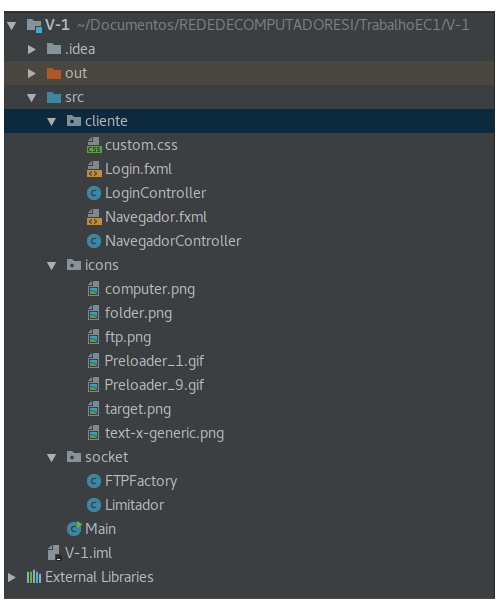
\includegraphics[width=.3\textwidth]{Imagens/001.png}
	\caption{ Imagem da Tela de Login.}
	\label{fig:01}
\end{figure}


Primeiramente, a classe Main é invocada, chamando a Scene do Login.fxml, o controle do login é responsável por fornecer o necessário para o FTPClient fazer a conexão.

\begin{lstlisting}

public class Main  extends Application{

@Override
	public void start(Stage stage) throws Exception {
	Parent root = FXMLLoader.load(getClasssingleton().getResource("/cliente/Login.fxml"));
	Scene scene = new Scene(root);
	stage.setScene(scene);
	stage.show();
}


public static void main(String[] args) {
	launch(args);

}

}

\end{lstlisting}

\begin{figure}[H]
	\centering
	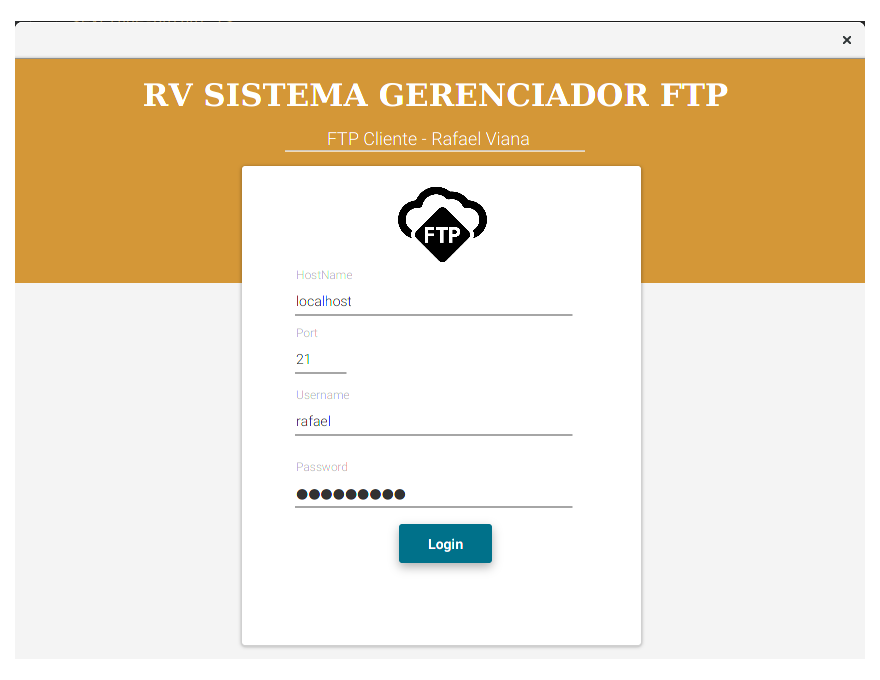
\includegraphics[width=.9\textwidth]{Imagens/01.png}
	\caption{ Imagem da Tela de Login.}
	\label{fig:02}
\end{figure}

Com a tela de login aberta o usuário entra com as informações login, senha, endereço do host, port do host mostrado no código abaixo e na Figura \ref{fig:02} .
\vspace{.4cm}
\begin{lstlisting}
private void login(ActionEvent event) {

	btnLogin.setVisible(false);
	imgProgress.setVisible(true);
	
	PauseTransition pauseTransition = new PauseTransition();
	pauseTransition.setDuration(Duration.seconds(3));
	pauseTransition.setOnFinished(ev -> {

try {
	
		int reply = FTPFactory.getInstance().FTPConecta(txtHostName.getText(),Integer.parseInt(txtHostPort.getText()),this.txtUsername.getText(),this.txtPassword.getText());
		System.out.println("Igual:" + reply);
		
		if (reply == 230) {
		
			btnLogin.getScene().getWindow().hide();
			completeLogin();
		
		} else {
		
			imgProgress.setVisible(false);
			btnLogin.setVisible(true);
			JOptionPane.showMessageDialog(null,"Erro Senha ou Usuário incorreto !!", "Erro ao Logar",JOptionPane.ERROR_MESSAGE);
		}

	} catch (IOException ex) {
		Logger.getLogger(LoginController.class.getName()).log(Level.SEVERE, null, ex);
	} catch (Exception ex) {
		Logger.getLogger(LoginController.class.getName()).log(Level.SEVERE, null, ex);
	}

});
  pauseTransition.play();
}

private void completeLogin() throws IOException {
	
	imgProgress.setVisible(false);
	Stage dashboardStage = new Stage();
	dashboardStage.setTitle("");
	Parent root = FXMLLoader.load(getClass().getResource("Navegador.fxml"));
	Scene scene = new Scene(root);
	dashboardStage.setScene(scene);
	dashboardStage.show();
	
}

\end{lstlisting}


Para realizar a comunicação entre as classes e o FTPClient da apache, criou-se uma classe Singleton chamada de FTPFactory onde a mesma utiliza uma getInstance de FTPClient, que pode ser chamada de qualquer classe, sem ter que ser instanciada novamente, o que irá ocasionar a perda da conexão FTP.

\begin{lstlisting}

public class FTPFactory {
	
	private final FTPClient ftp;
	private TreeItem<FTPFile> file;
		
	private FTPFactory() {
			this.ftp = new FTPClient();
	}
	
	public static FTPFactory getInstance() {
	
		return FTPFactoryHolder.INSTANCE;
	}


	/**
	* Classe privada que armazena a única instância de FTPFactory.
	*/
	
	private static class FTPFactoryHolder {
	
		private static final FTPFactory INSTANCE = new FTPFactory();
	}


	public FTPClient getFTP() {
		return this.ftp;
	}


	public boolean Excluir(FTPFile file) {
	try {
			if (file.isDirectory()) {
				System.out.println(file.getLink());
				return ftp.removeDirectory(file.getLink());
			} else {
				System.out.println(file.getLink());
				return ftp.deleteFile(file.getLink());
			}
	} catch (IOException e) {
		e.printStackTrace();
		}	
		return false;
	}


	public int FTPConecta(String host, int port, String user, String pwd) throws Exception {
		int reply;
		ftp.connect(host, port);
		reply = ftp.getReplyCode();
		if (!FTPReply.isPositiveCompletion(reply)) {
			ftp.disconnect();
			throw new Exception("Exception in connecting to FTP Server");
		}
		ftp.login(user, pwd);
		reply = ftp.getReplyCode();
		ftp.setFileType(FTPClient.BINARY_FILE_TYPE);
		ftp.enterLocalPassiveMode();
		ftp.setAutodetectUTF8(true);
		return reply;
	}


	public void disconnect() {
		if (this.ftp.isConnected()) {
		try {
			this.ftp.logout();
			this.ftp.disconnect();
			} catch (IOException f) {
	
			}
	    }
	}
}	

\end{lstlisting}

Após a classe login em conjunto com a classe FTPFactory, validar os dados de usuário a tela de navegação é aberta, essa tela nada mais é do que um conjunto de botões em uma Grid à esquerda um ToolBar no top e um TreeView do JavaFX no centro para poder navegar pela estutura dos diretórios.

\begin{figure}[H]
	\centering
	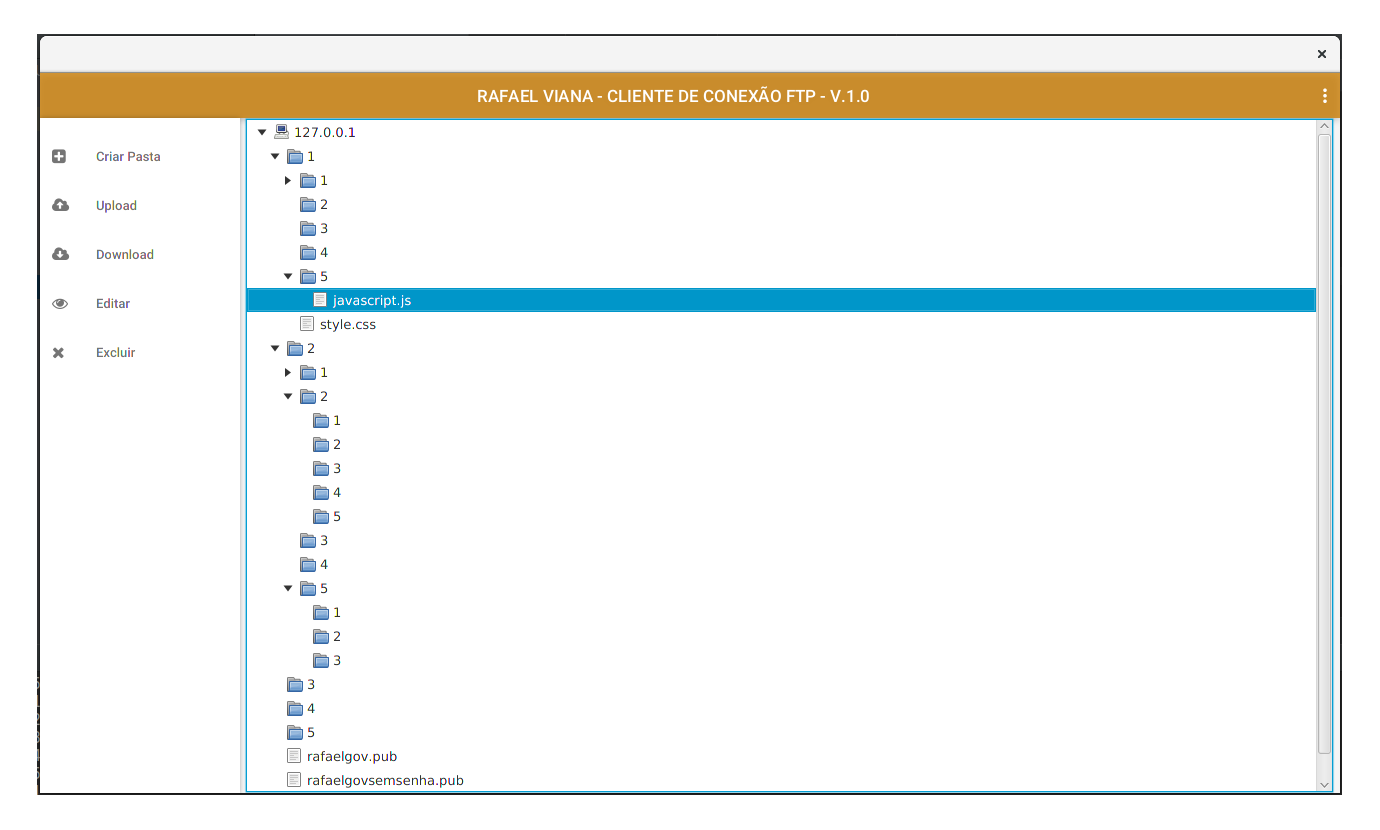
\includegraphics[width=0.8\textwidth]{Imagens/02.png}
	\caption{ Imagem da Tela de Navegação.}
	\label{fig:03}
\end{figure}


Toda lógica de abastecimento da TreeView e a criação dos TreeItem utilizados na TreeView estão no método Navegacao(), pertencente a classe NavegadorController, o mesmo chama o método CarregarFiles(), que tem a obrigação de criar recursivamente a partir dos arquivos que estão no servidor FTP, os TreeItem<FTPFile> que são encadeando-os e lançandos na TreeView, facilitando assim a navegação pelos diretórios.

Para melhor leitura os métodos implementados pelos botões foram removidos, porém podem ser veficados na classe NavegadorController no código fonte. As funções que os mesmo exercem são com base nos comandos implementados no FTPClient da Apache sendo estes:
\begin{enumerate}
\item {Criar Pasta} makeDirectory(String caminho)	
	
Este método exige um caminho do diretório remoto para criar uma pasta no mesmo.  
	
\item {Criar Arquivo} makeDirectory()	
	
Este método exige um caminho do diretório remoto para criar um arquivo no mesmo.

\item {Upload Arquivo } storeFile(String caminho, InputStream local)	

Este método exige um caminho do diretório remoto e um InputStream local, que indique o arquivo desejado.

\item {Download } retrieveFile(String caminho, OutputStream local)	

Este método exige um caminho do diretório remoto que tenha o arquivo e OutputStream para o local de destino do arquivo.

\item {Editar} rename(String nomeAtual, String novoNome)	

Este método exige o nome do diretório remoto que deseja alterar e o novo nome para o mesmo.  

\item {Excluir} removeDirectory(String diretorioRemoto) ou  deleteFileString(String arquivoRemoto) 

Para excluir foram utilizados dois métodos, um para deletar as pastas removeDirectory(String caminhoRemoto) e outro para arquivos deleteFileString(String caminhoRemoto).

\end{enumerate}

\begin{lstlisting}

private void Navegacao() throws IOException {
	FTPFile files[];
	TreeItem<FTPFile> treeRoot;
	files = FTPFactory.getInstance().getFTP().listFiles();
	Tree.setEditable(true);
	if (files != null && files.length > 0) {
		files[0].setRawListing(FTPFactory.getInstance().getFTP().getPassiveHost());
		treeRoot = CarregarFiles(files[0], true);
	} else {
		FTPFile file = new FTPFile();
		file.setType(FTPFile.DIRECTORY_TYPE);
		file.setLink(FTPFactory.getInstance().getFTP().printWorkingDirectory());
		file.setRawListing(FTPFactory.getInstance().getFTP().getPassiveHost());
		treeRoot = new TreeItem<>(file, new ImageView(computador));
	}
	
	Tree.getSelectionModel().select(treeRoot);	
	Tree.setRoot(treeRoot);
	
	//Os Botões ADD,RENAME,DELETE,UPLOAD e DOWNLOAD estão nessa classe, foram retirados para um melhor entendimento do código.

}


public TreeItem<FTPFile> CarregarFiles(FTPFile directory, boolean v) throws IOException {
	
	TreeItem<FTPFile> root;

	if (v) {
		directory.setType(FTPFile.DIRECTORY_TYPE);
		directory.setLink(FTPFactory.getInstance().getFTP().printWorkingDirectory());
		root = new TreeItem<FTPFile>(directory, new ImageView(computador));
    } else {
		root = new TreeItem<FTPFile>(directory, new ImageView(pasta));
	}
	root.setExpanded(true);
	FTPFile[] files = FTPFactory.getInstance().getFTP().listFiles();
	for (FTPFile f : files) {
		System.out.println("Carregando .. " + f.getName());
	    if (f.isDirectory()) {
			FTPFactory.getInstance().getFTP().changeWorkingDirectory(f.getName());
			f.setLink(FTPFactory.getInstance().getFTP().printWorkingDirectory());
			root.getChildren().add(CarregarFiles(f, false));
		} else {
		f.setLink(FTPFactory.getInstance().getFTP().printWorkingDirectory() + separador + f.getName());
		root.getChildren().add(new TreeItem<FTPFile>(f, new ImageView(this.arquivo)));
		}
	}
	FTPFactory.getInstance().getFTP().changeToParentDirectory(); 
	return root;
}

\end{lstlisting}

Um dos objetivos do trabalho é limitar o cliente FTP, fazendo com que usuários que utilizam o sistema possam criar 5 pastas e 2 arquivos por diretório, sendo que poderão criar no máximo 3 níveis de diretórios.

A classe Limitador do pacote socket é responsável por fazer a armazenagem da quantidade máxima de pastas e arquivos. Sendo utilizada na classe NavegadorController do pacote cliente, em conjunto dos métodos limiteArquivo(), limitePasta()  e limiteNivel().
 
 \begin{lstlisting}
public class Limitador {

	private int p;
	private int a;
	
	public Limitador(int p, int a) {
		this.p = p;
		this.a = a;
	}
	
	public int getMP() {
		return p;
	}
	
	public int getMA() {
		return a;
	}

}

// Os métodos abaixo pertencem a classe NavegadorControoler

private boolean limiteArquivo() throws IOException {
	int num = FTPFactory.getInstance().getFTP().listDirectories().length;
	int numa = FTPFactory.getInstance().getFTP().listFiles().length - num;
	return numa < limite.getMA();
}

private boolean limitePasta() throws IOException {
	int num_diretorios = FTPFactory.getInstance().getFTP().listDirectories().length;
	return num_diretorios < limite.getMP();
}

private int limiteNivel() throws IOException {
	int num = FTPFactory.getInstance().getFTP().printWorkingDirectory().split("/").length;
	return num;
}


\end{lstlisting}
	Para deletar uma pasta deve-se utilizar o método removeDirectory(Caminho), ou para deletar um arquivo utiliza-se o método deleteFile(Caminho) do FTPClient Apache. Porém para deletar uma pasta que contém N sub pastas deve-se percorrer recursivamente as pastas, até a folha mais baixa e seguir apagando debaixo para cima cada pasta ou arquivo, recursivamente pelo método DeletarRecursivo(TreeItem), implementado na classe NavegadorController.  
\begin{lstlisting}

public boolean DeletarRecursivo(TreeItem<FTPFile> a) {
	boolean flag = false;
	
	if (a.getChildren().isEmpty()) {
		if (FTPFactory.getInstance().Excluir(a.getValue())) {
			return true;
		}
	}else {
	
		for (TreeItem<FTPFile> iterator: a.getChildren()){
			DeletarRecursivo(iterator);
		}
		
		if (FTPFactory.getInstance().Excluir(a.getValue())) {
			return true;
		}
	}
	return false;
}
\end{lstlisting}
	Após a renomeação de um TreeItem<FTPFile> da TreeViw, foi preciso modificar recursivamente os TreeItem<FTPFile> filhos, pelo método RenameRecursivao(TreeItem<FTPFile> a), esse método notifica os filhos mundando assim o link dos mesmos.
\begin{lstlisting}
public void RenameRecursivao(TreeItem<FTPFile> a) {
	String novolink;
	for (Iterator<TreeItem<FTPFile>> iterator = a.getChildren().iterator(); iterator.hasNext(); ) {
		TreeItem<FTPFile> c = iterator.next();
		novolink = a.getValue().getLink() + separador + c.getValue().getName();
		c.getValue().setLink(novolink);
		if (!c.getChildren().isEmpty()) {
			RenameRecursivao(c);
		}
	}
}
\end{lstlisting}

\section{Testes}
Foram realizados testes funcionais para correções de erros, na implementação. Para uma maior segurança foram realizados testes nos métodos de criação de pastas e arquivos, exclusão de pastas e arquivos, adicionar arquivos e pastas, upload de arquivos, renomeação arquivos e pastas, download de arquivos e exclusão de diretório inteiro.

 \bibliography{bibli}

\end{document}


